%----------------------------------------------------------------------------------------
%	PACKAGES AND DOCUMENT CONFIGURATIONS
%----------------------------------------------------------------------------------------
\documentclass[11pt]{article}
\usepackage{amsmath} % Required for some math elements
\usepackage{hyperref} 
\usepackage{xcolor}
\usepackage{lipsum} 
\usepackage{cite}
\usepackage{graphicx} % Required for the inclusion of images
\usepackage{algorithmic}
\usepackage{array}
\usepackage{bookmark}
\usepackage{listings}
\usepackage{amssymb}
\usepackage{enumitem}
\usepackage[margin=24mm]{geometry}
\usepackage[caption=false, font=footnotesize]{subfig}
\usepackage{multirow}
\usepackage[active,tightpage]{preview}

\renewcommand{\PreviewBorder}{1in}
\newcommand{\Newpage}{\end{preview}\begin{preview}}

\newlist{steps}{enumerate}{1}
\setlist[steps, 1]{label = Step \arabic*:}

\hypersetup{ %color attributes of citation, link, etc.
    colorlinks=true,
    linkcolor=blue,
    filecolor=gray,      
    urlcolor=blue,
    citecolor=blue,
}


\definecolor{mGreen}{rgb}{0,0.7,0.5}
\definecolor{mWhite}{rgb}{0.9,0.9,0.9}
\definecolor{mGray}{rgb}{0.5,0.5,0.5}
\definecolor{mPurple}{rgb}{0.58,0,0.82}
\definecolor{backgroundColour}{rgb}{0.0,0.0,0.1}

\lstdefinestyle{Cstyle}{
    backgroundcolor=\color{backgroundColour},   
    commentstyle=\color{mGreen},
    keywordstyle=\color{magenta},
    numberstyle=\tiny\color{mGray},
    stringstyle=\color{mPurple},
    basicstyle=\footnotesize\color{mWhite},
    breakatwhitespace=false,         
    breaklines=true,                 
    captionpos=b,                    
    keepspaces=true,                 
    numbers=left,                    
    numbersep=5pt,                  
    showspaces=false,                
    showstringspaces=false,
    showtabs=false,                  
    tabsize=4,
    language=C
}


\newcommand{\matlab}{\textsc{Matlab }} %very important and totally necessary addition

\newcommand\Item[1][]{%
  \ifx\relax#1\relax  \item \else \item[#1] \fi
  \abovedisplayskip=0pt\abovedisplayshortskip=0pt~\vspace*{-\baselineskip}}
  %----------------------------------------------------------------------------------------
%	DOCUMENT INFORMATION
%----------------------------------------------------------------------------------------
 
\title{ECEN301 : Embedded Systems \\ Lab 2 Submission}
\author{Daniel Eisen : 300447549}
\date{\today}

\begin{document}
\begin{preview}
\maketitle
%----------------------------------------------------------------------------------------
%	DOCUMENT CONTENT
%----------------------------------------------------------------------------------------
\section{Objectives}
This lab demonstrated the use of the analogue to digital convertor onboard the 8051 as well as displaying data to a discrete LCD display. Using that as a base we covered analogue sensor input (in the form of a thermistor) as well as calibration, linearization and unit conversion. Side effects of this was encountering the limitations that an embedded engineer must overcome, such as small stack size, peripheral type limitations etc.

\section{Methodology}
        \subsection{Introduction}
        This lab requires the 8051, the LCD display (control to P4, data to P0), and breadboard module with a variable voltage divider module attached. As with the last lab, the programs were developed and compiled to a hex file with Atmel Studio and the included 8051 library and lab modules library.
        
        
        Initially LCD control was tested with basic IO, then familiarising ourselves with the ADC by designing a basic voltmeter, then finally, with more complexity a temperature measurement program was designed and calibrated.   

        \subsection{LCD Display}
        \begin{center}
                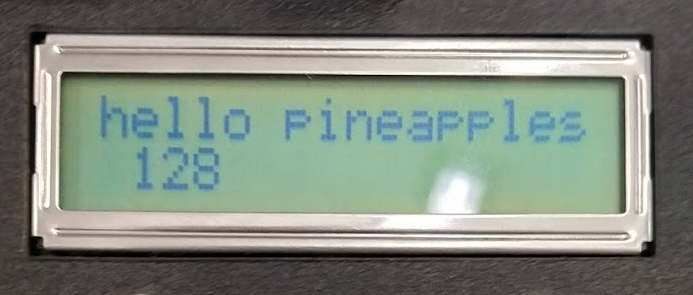
\includegraphics[width=0.65\textwidth]{res/LCD0.jpg}

                \textit{Fig. 1 LCD text and number}
        \end{center}

        First connecting the module to the $\mu$C (control to P4, data to P0), a program can then be written to interface with it. This allows for much more readable and diverse program output that can be read with out via the 7-seg or LEDs on the IO module. To be able to write to the LCD panel, the ECEN301LibSDCC.h library is used to abstract the interfacing specifics away from the main control flow of the program. \\

        To be able to write multiple data types to the LCD the std.io library can be used, specifically the \texttt{sprintf} function for formatting an char pointer variable to be printed later. \\

        On the subject of this char pointer, this is a significant cause of stack memory usage so during the lab it was found that anything over a size of 32 was uncompilable so keeping to 16 was necessary for larger programs. Though a size 32 array was needed for a 2 lines display. \\
        
        To prevent flashing a delay used to hold the current state within the loop.
        \lstinputlisting[language=C,style=CStyle]{res/lcd.c}

        \subsection{ADC}
        \begin{center}
                \fbox{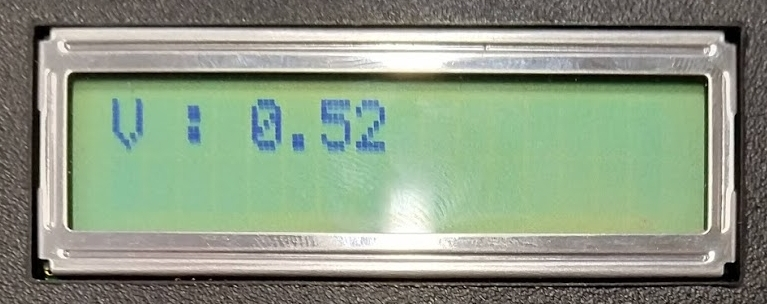
\includegraphics[width=0.45\textwidth]{res/vmeasure0.jpg}
                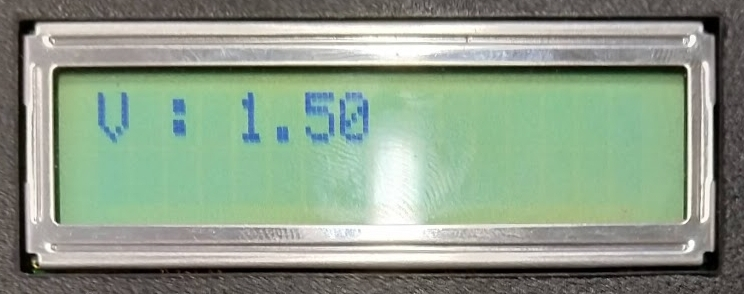
\includegraphics[width=0.45\textwidth]{res/vmeasure1.jpg}}
                \fbox{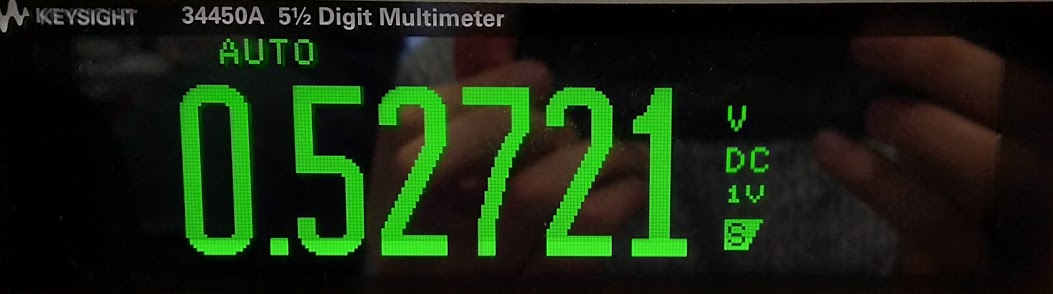
\includegraphics[width=0.45\textwidth]{res/vactual0.jpg}
                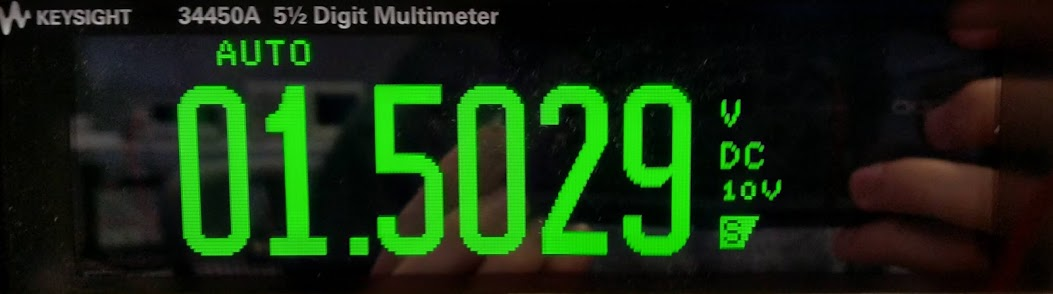
\includegraphics[width=0.45\textwidth]{res/vactual1.jpg}}

                \textit{Fig. 2 Comparison between reading and "true" value}  
        \end{center}

        The main purpose of the analog converters is to convert conditioned analog signals into digital data so that the microcontroller system can process them for display, calculations, and analysis etc.
        To do this in the 8051, this is controlled via the ADCON and ADCF special function registers registers. \\

        
        \begin{center}
                \fbox{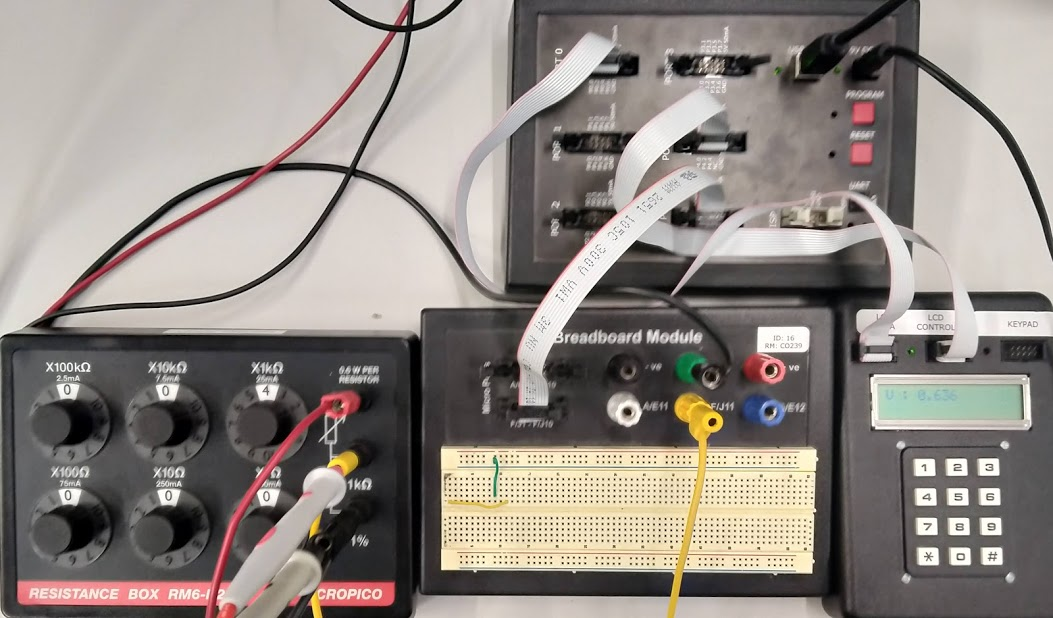
\includegraphics[width = 0.5\textwidth]{res/voltmeter.jpg}}
        \end{center}
        The setup for our use case is a voltage meter, utilising a voltage divider of the reference voltage as the analog input signal. This is seen above. The voltage is varied by changing $R_{total}$ with the variable resistance module.
        To setup the ADC for take and convert and external input, ADCF is used to select input channel, then ADCON to enable ADC, set CPU into pseudo idle, and start the conversion.
        Pseudo Idle mode, is a reduces the CPU noise to a state where the last 2 bit of the 10bit ADC are usable.
        After this, the end of conversion flag must be reset in software, and the resulting conversion can be read from ADDH and ADDL.\\
        
        The procedure of calibrating this digital reading to a displayable voltage value is as follows.
        $$voltage = ADC_{sample} * V_{ref} / 2^{10}$$
        This can then be displayed to LCD, but due to being unable to writing floats to a string the reading must be split across the decimal place and displayed "separately".

        \lstinputlisting[language=C,style=CStyle]{res/volt.c}

        \subsection{Temperature}
        For a more complex and practical demonstration of the ADC, we implemented a Temperature sensor. Using a thermistor is as a temperature dependant resistance as an analog sensor input to the ADC. From then it can be calibrated with known temperatures and characterised. 
        \subsubsection*{Setup}
        Leaving the modules in same configuration as before, with the breadboard suppling the ADC input, with the same LCD output except in this case replacing the voltage divider the thermistor and matched resistance. At room temperature the nominal resistance was measured at ~10k so this is what was used as the second resistance.

        \subsubsection*{Calibration}
        The value of the thermistors resistance cannot be directly as temperature, so its it must be characterised and translated into a temperature. 

        Using a thermometer and range of temperatures I correlated the ADC value and the measure value. This is seen to be non linear so to make it more usable linearization is applied to spilt the curve into two regions and fitting a linear curve to them to get an equation to translate the ADC reading to a temperature

        \begin{center}
                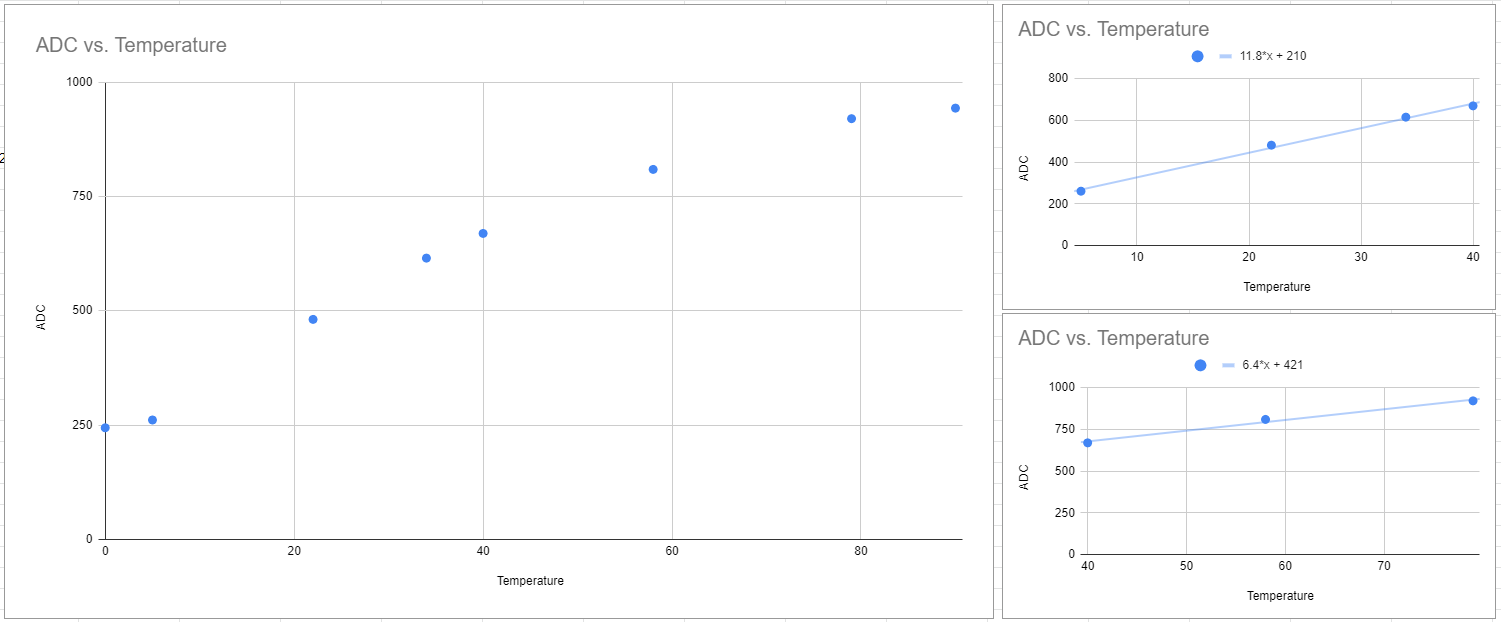
\includegraphics[width=0.6\textwidth]{res/tempFIT.png}

                \textit{Fig. 3 Thermistor Charactisaion}
        \end{center}
        
        
        \subsubsection*{Program and output}
        \begin{center}
                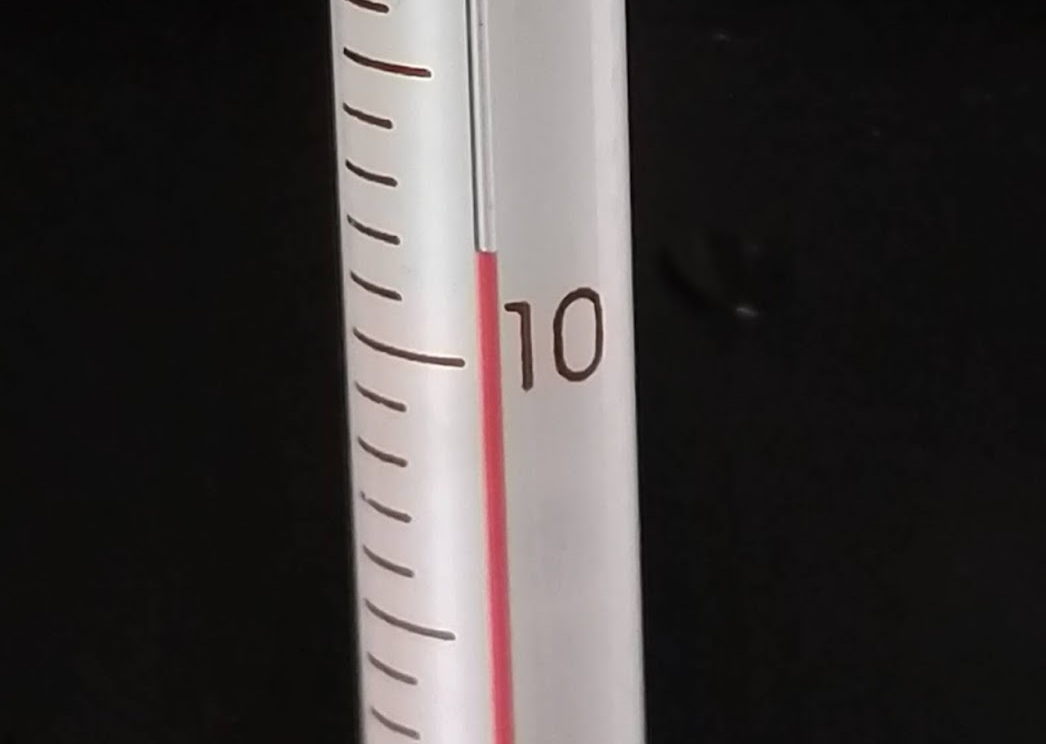
\includegraphics[width=0.25\textwidth]{res/temp0.jpg}
                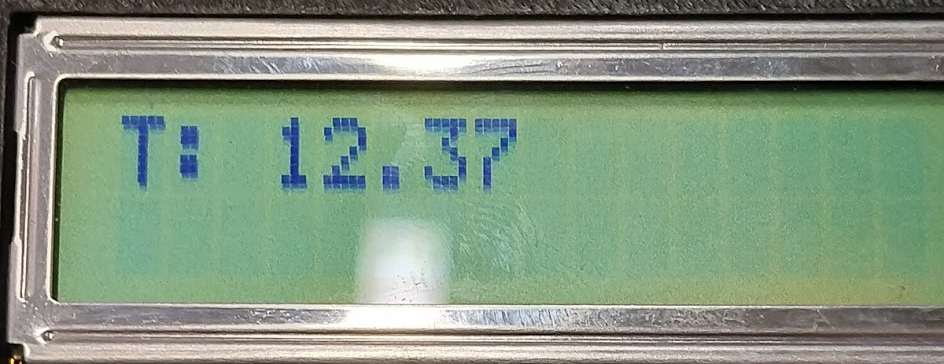
\includegraphics[width=0.45\textwidth]{res/tempADC0.jpg}

                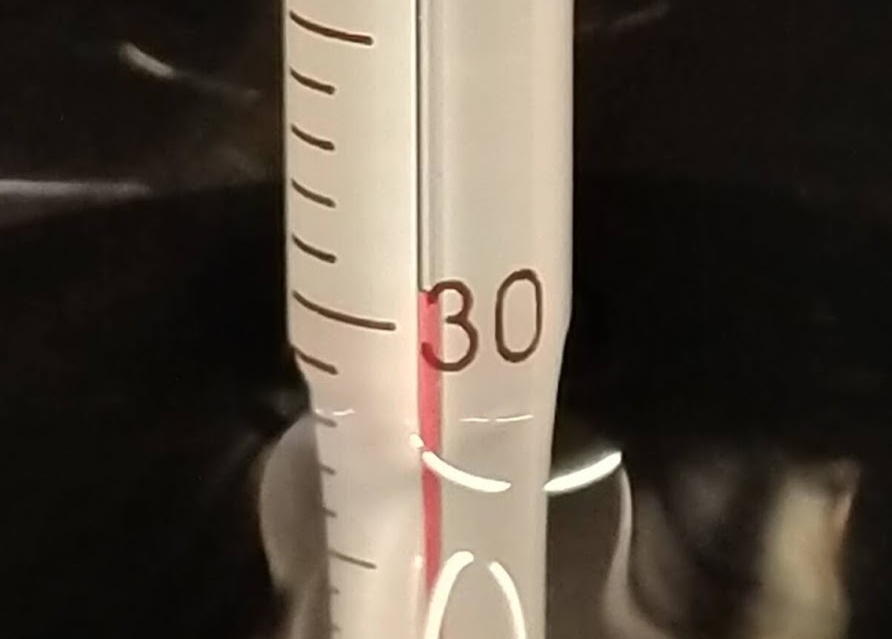
\includegraphics[width=0.25\textwidth]{res/temp1.jpg}
                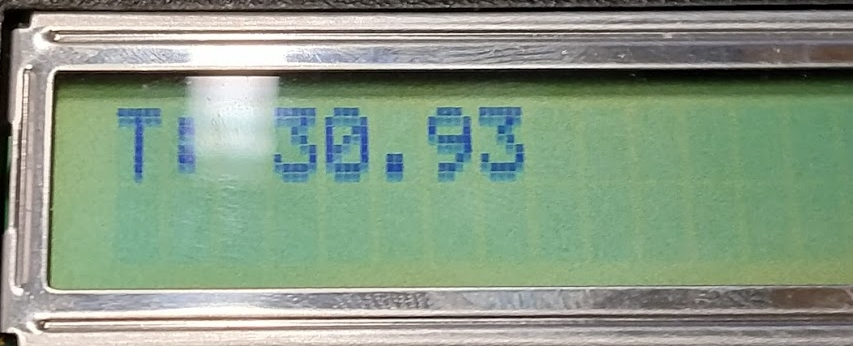
\includegraphics[width=0.45\textwidth]{res/tempADC1.jpg}
        \end{center}

        As seen above, the characterised equations when implemented into the program work to a reasonable accuracy with a normal operating range.

        In the implemented program, there is a check to switch from one region to the other.

        When extending the functionality, I encountered multiple issue regard stack memory space. Due to the lack of floating point support I found myself having to store more and more temp variables for each side of the decimal place. The sliding average worked well and is implemented but the necessary array didn't help with stack space. This is why I didn't get SD and min max working.

        How I would implement it now would, instead of floats, work with scaled (x100) ints for the value then use a modulus method to split them. ie temp = 3042: temp/100 would be 30 and temp\%100 would be 42 and print those either side of the decimal point.
        
        This would enable a much better usage of stack space, clean up the readability and increase performance. 

        \lstinputlisting[language=C,style=CStyle]{res/temp.c}
\section{Questions}
\begin{enumerate}
        \item \textit{Explain what all of the bits in the ADCON and ADCF registers mean?} \\
        \begin{itemize}
                \item ADCF is the 'ADC Configuration' register. Setting one of the bits in this register enable the corresponding pin on Port 1 for the input to the ADC, (Clearing sets it back to standard IO).
                \item ADCON is the control register for the ADC:
                \begin{itemize}
                        \item Bit 7 is reserved
                        \item Bit 6, set this to enable "pseudo idle mode." Basically putting the CPU into sort of sleep/low actively mode that allow the full 10bits of data from ADC to be used. This is due to the reduction in CPU noise.
                        \item Bit 5 enables/standbys the ADC. If code doesn't use the ADC clearing this can save power.
                        \item Bit 4 is a flag that is set when the ADC and finished doing a reading, this needs to be cleared by your code.
                        \item Bit 3 is used to start the conversion, this cleared afterward by the hardware.
                        \item Bit 2:0 are used to select between the 8 input channels
                \end{itemize} 
        \end{itemize}

\end{enumerate}

\end{preview}
\end{document}